

\documentclass{article}
\usepackage[spanish]{babel}
\usepackage{graphicx}
\usepackage{listings}
\setlength{\parindent}{0pt}
\setlength{\parskip}{3mm}
\usepackage[numbers]{natbib}
\usepackage{color}
\usepackage{booktabs}
\usepackage{subfigure}
\usepackage{pdfpages}



\begin{document}

\title{Portafolio}
\author{Dayli Machado (5275)}
\date{\today}
\maketitle

\section{Introdución}

A continuación se muestra el portafolio con las rectifaciones realizadas en las tareas de clases.

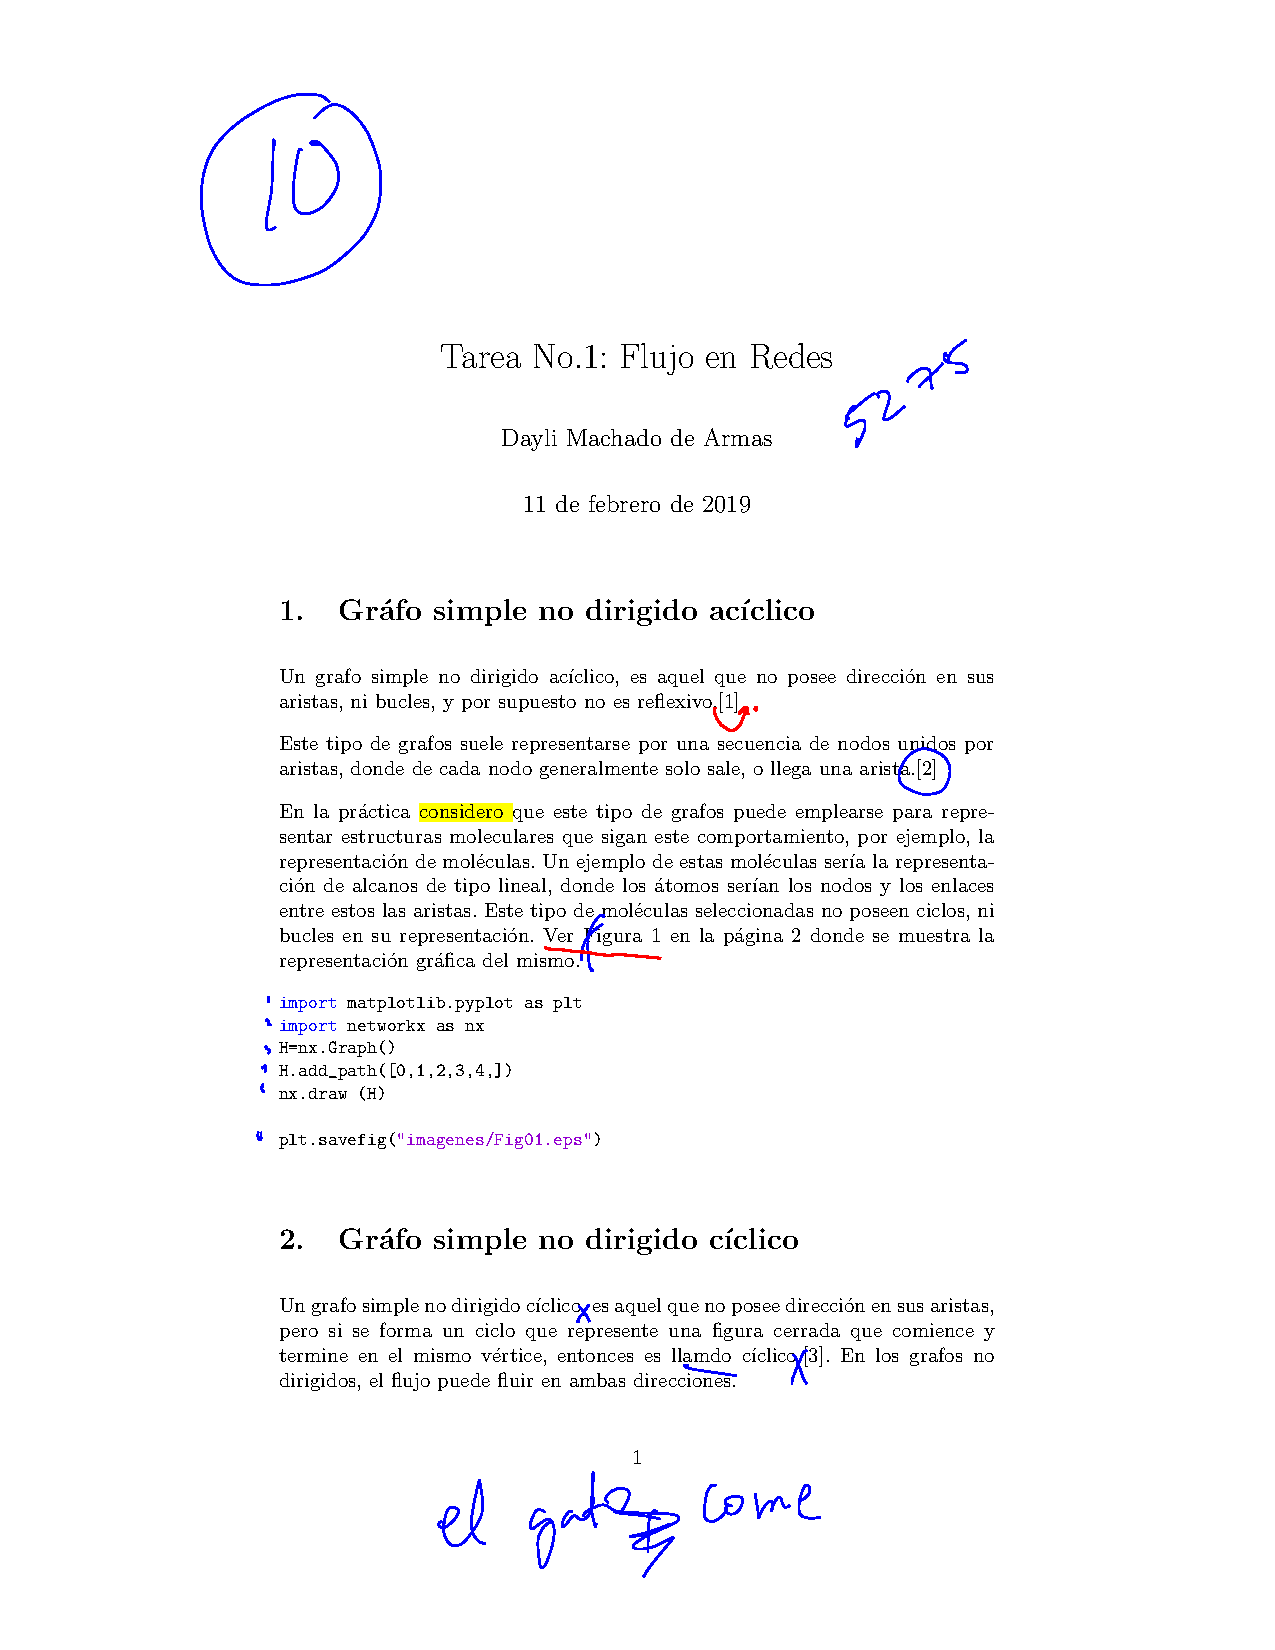
\includepdf[pages=1-22]{pdfrevisados/5275-1.pdf}
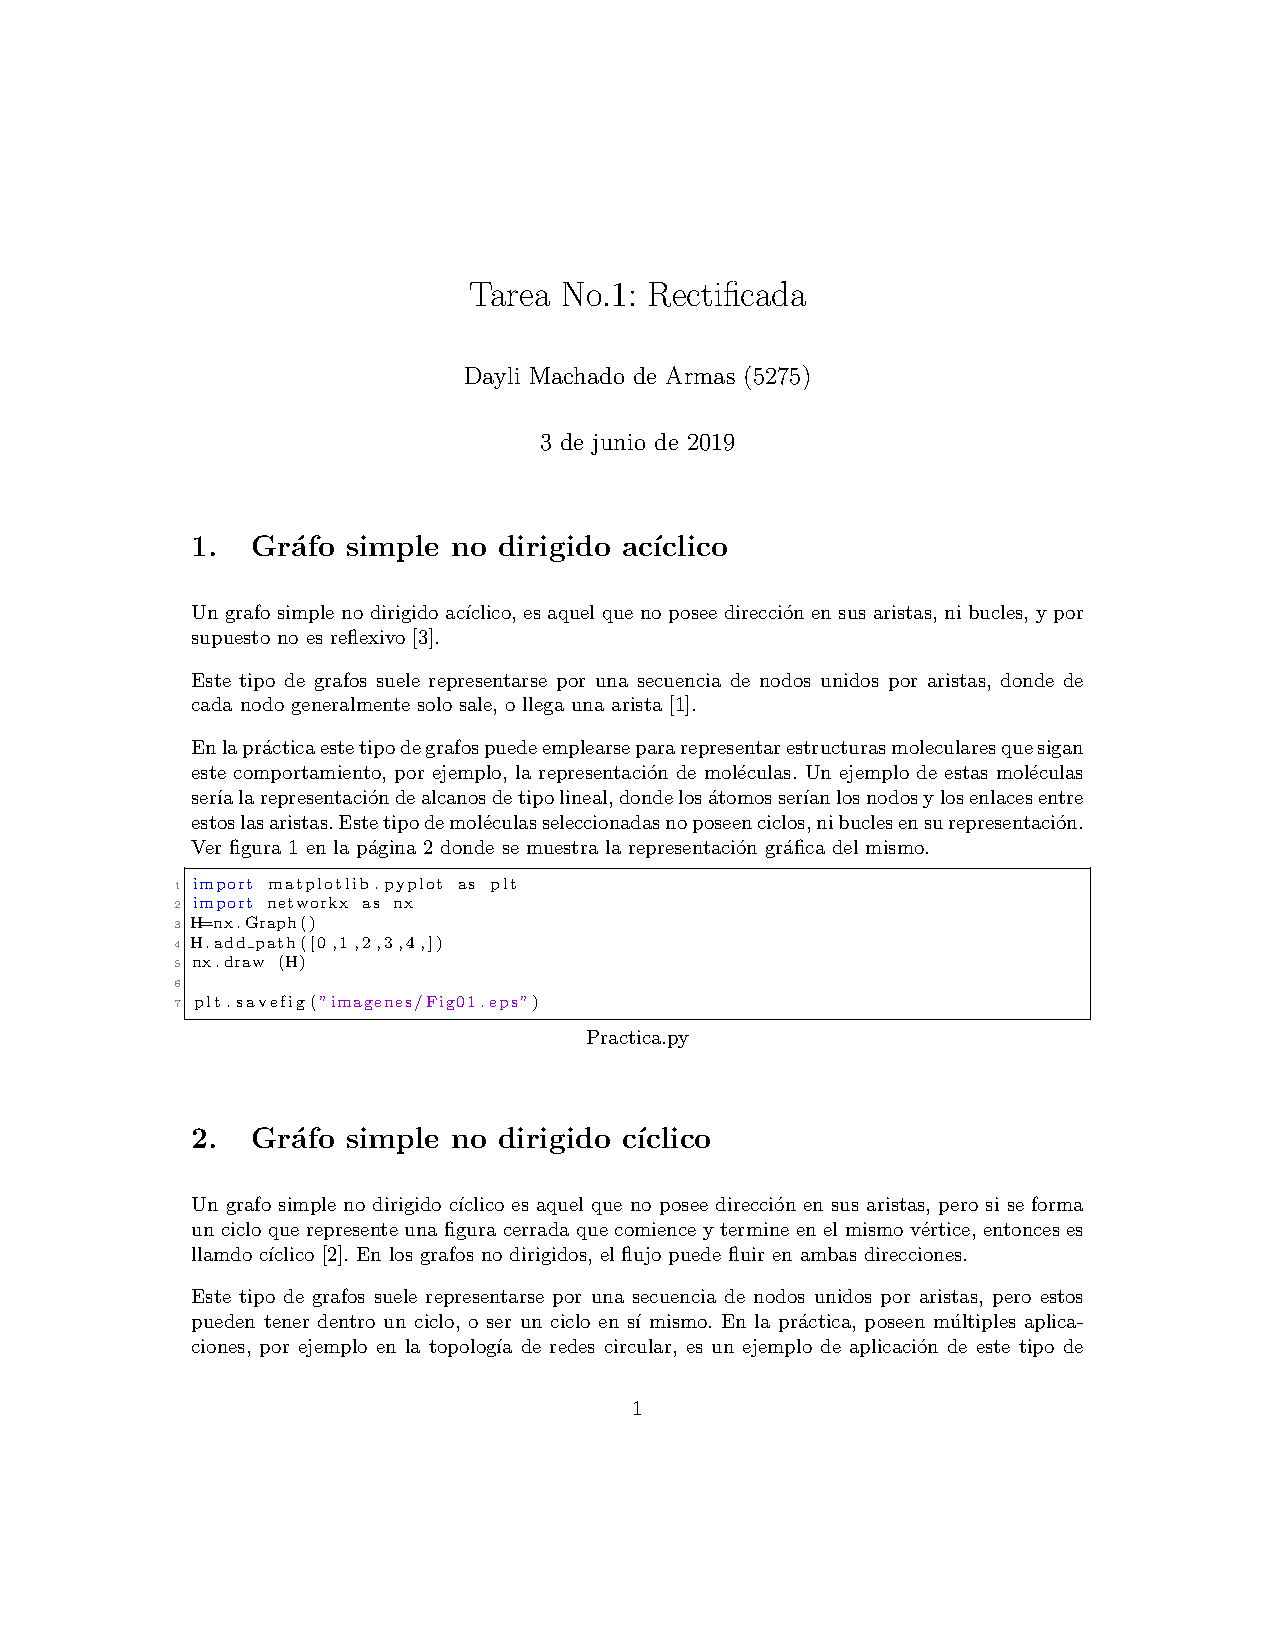
\includepdf[pages=1-19]{pdfrectificados/Tarea1_Rectificada.pdf}

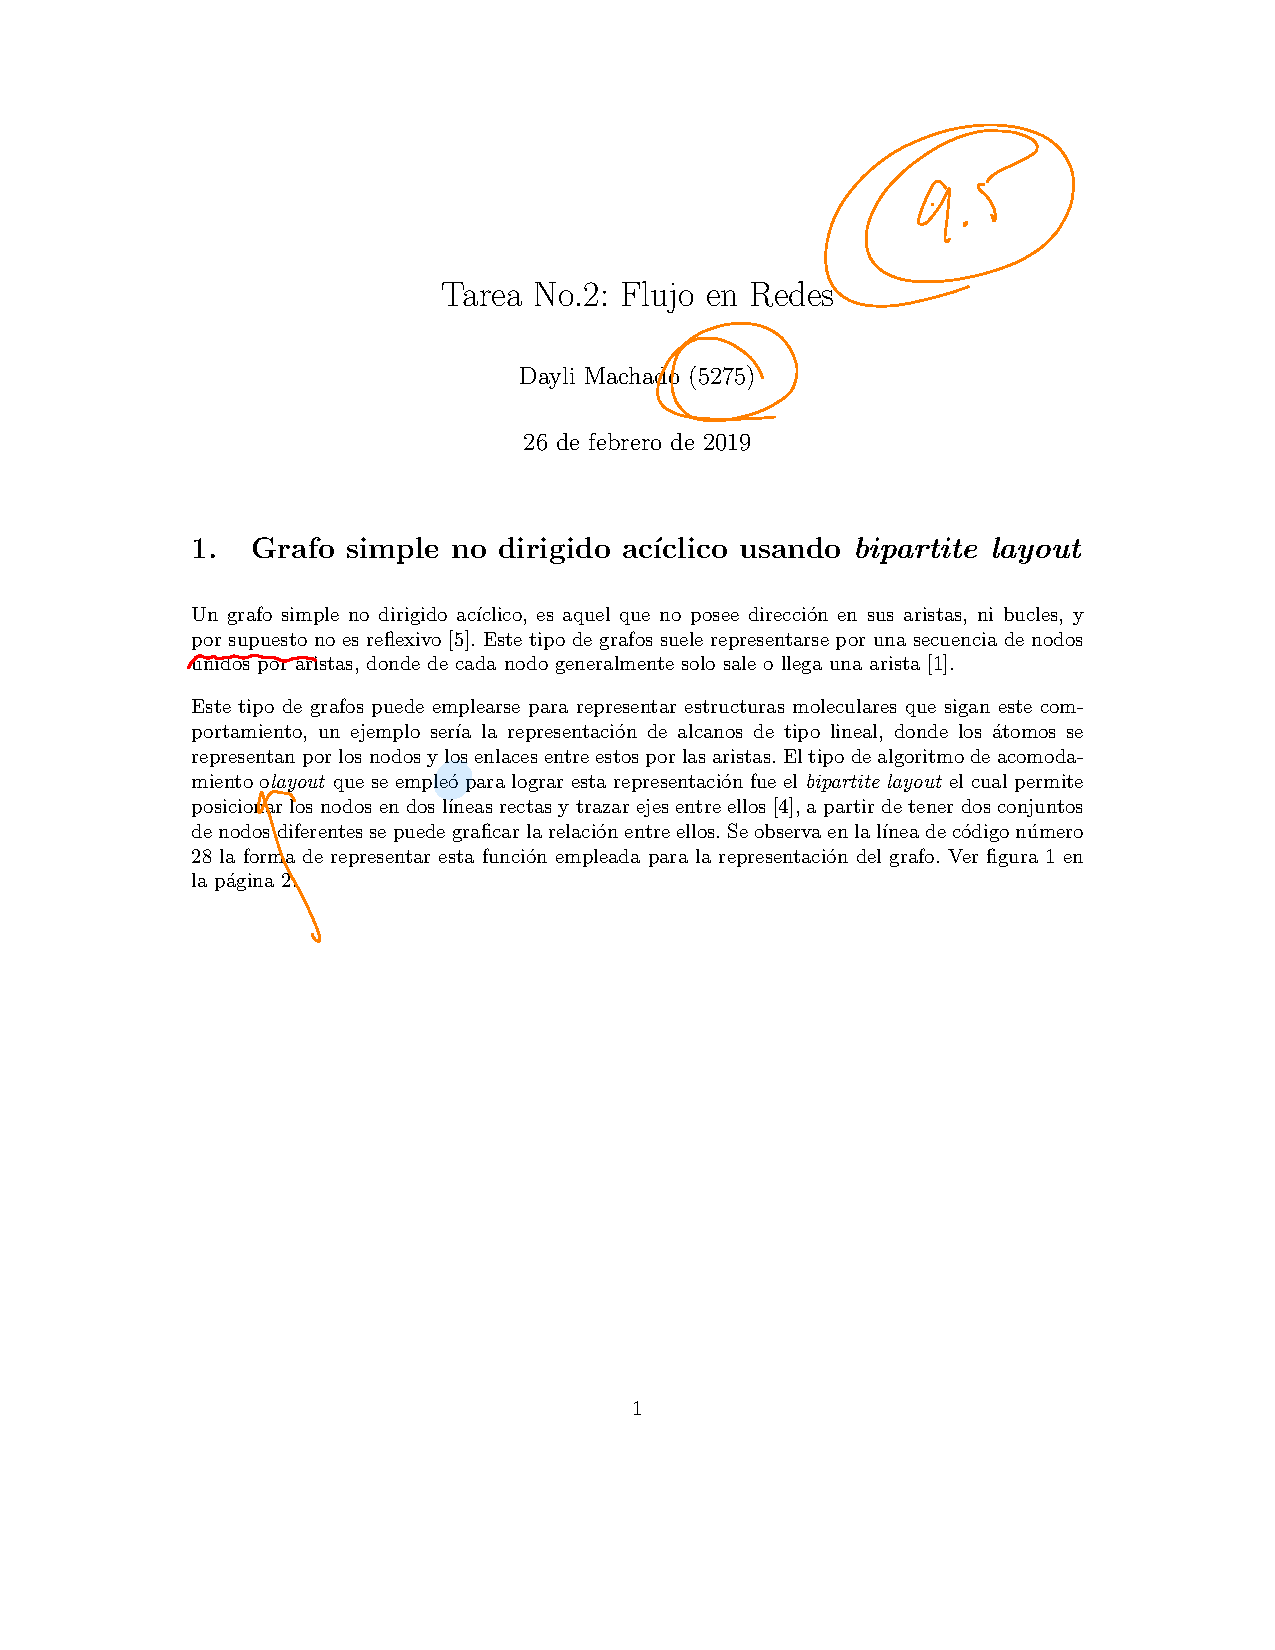
\includepdf[pages=1-27]{pdfrevisados/5275-2.pdf}
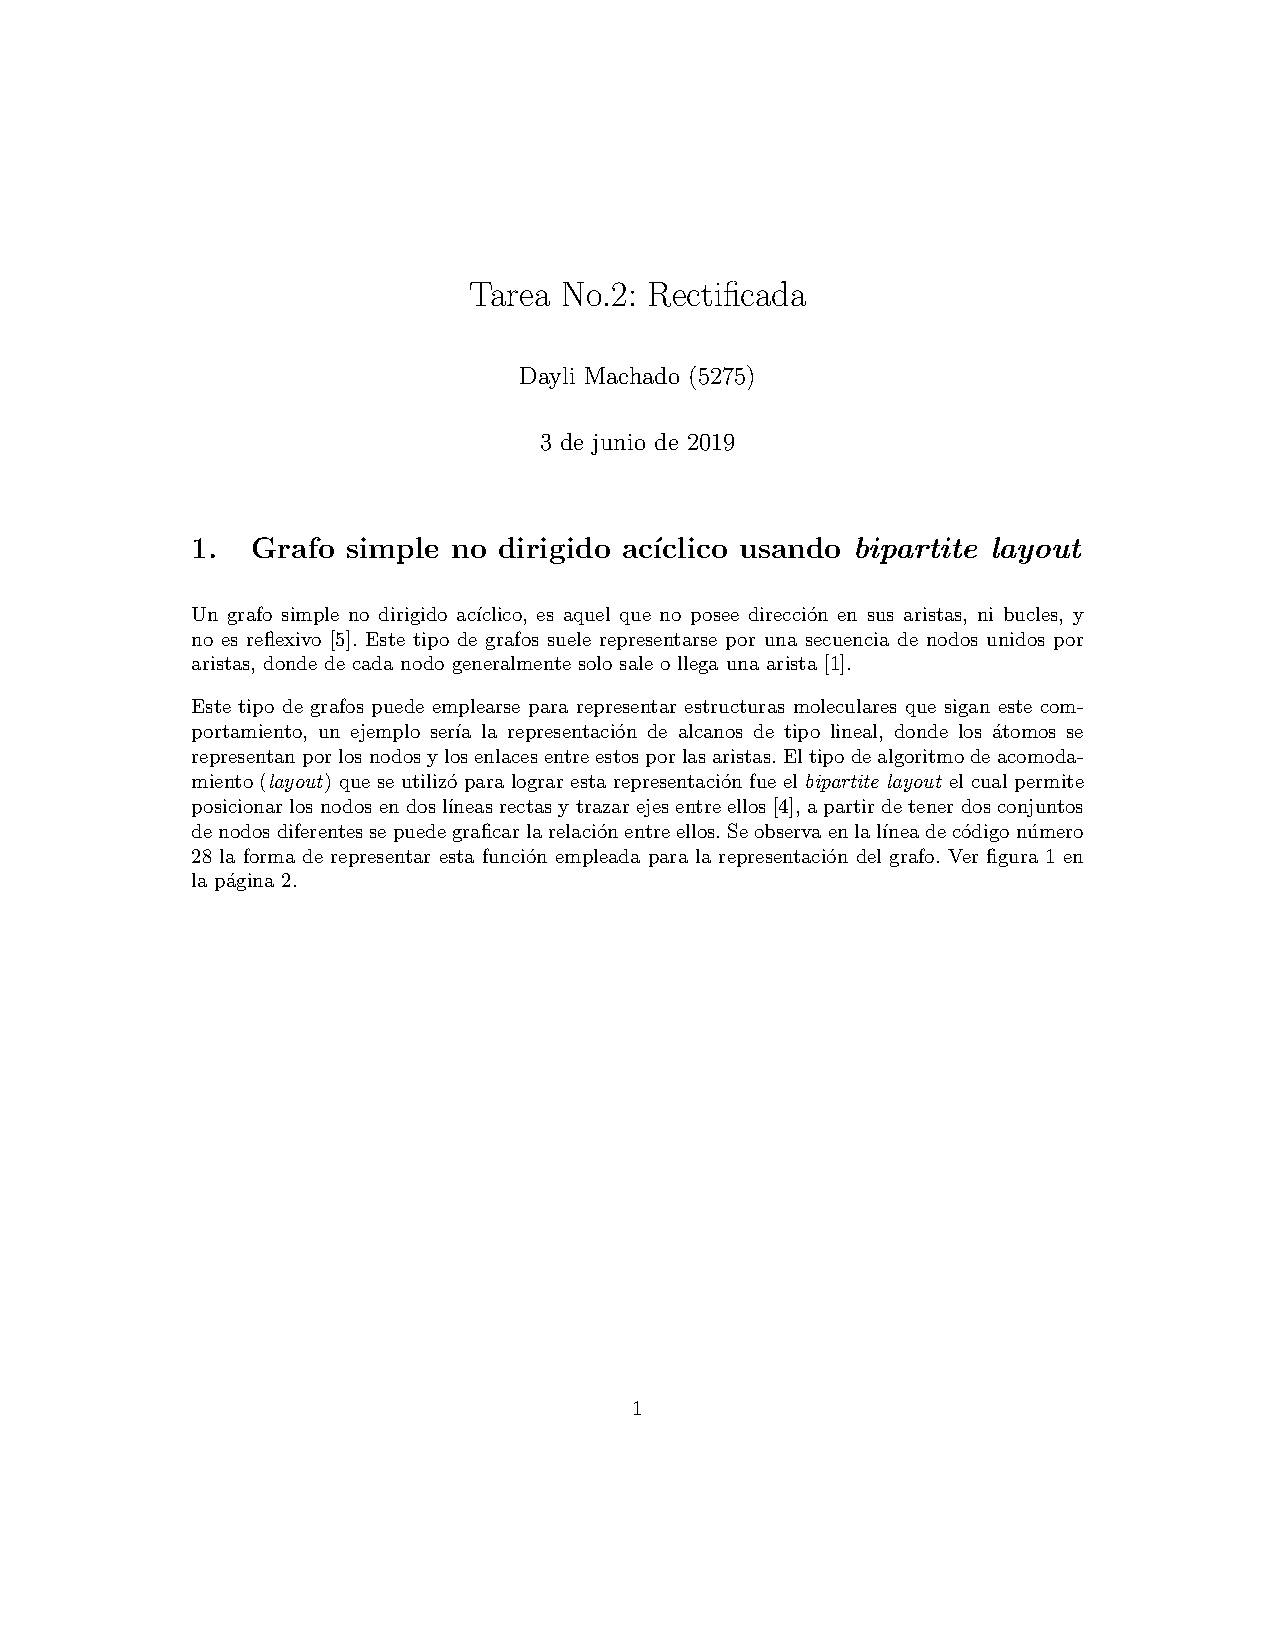
\includepdf[pages=1-27]{pdfrectificados/Tarea2_Rectificada.pdf}

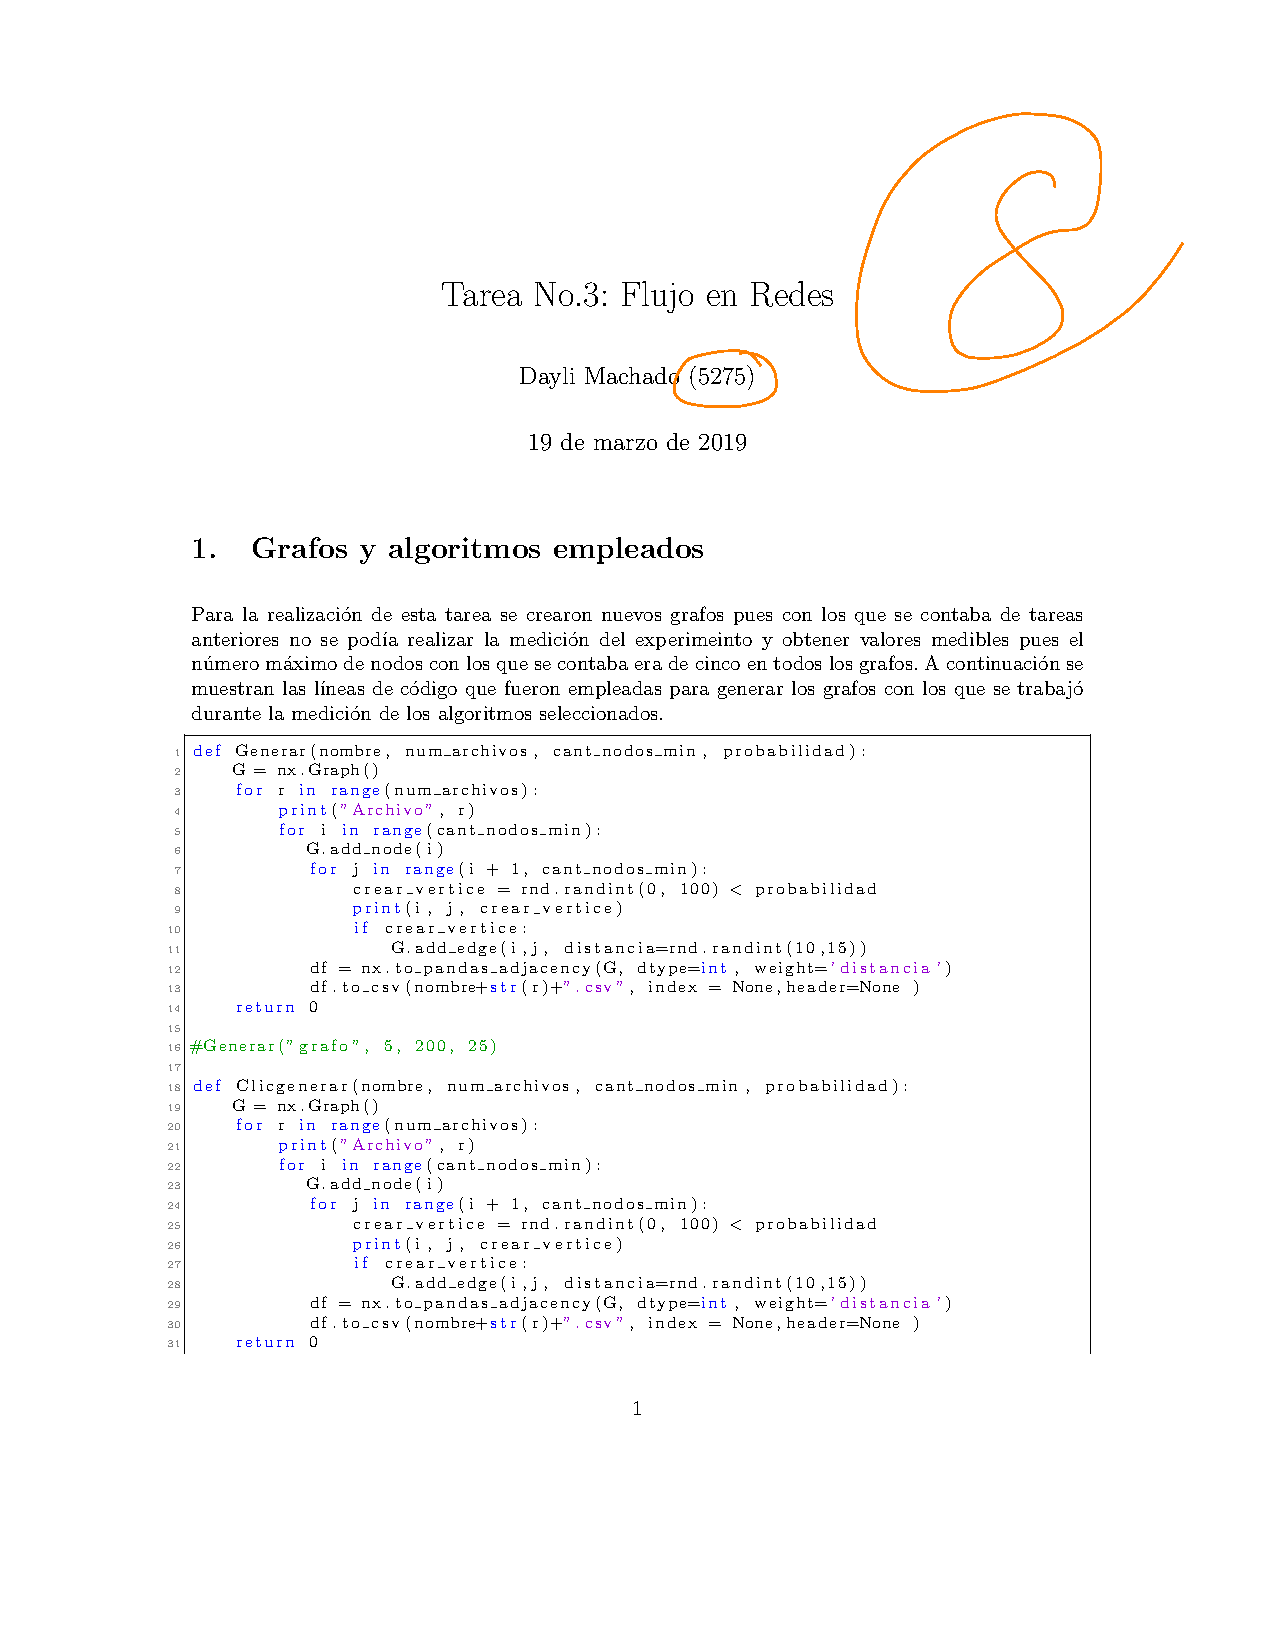
\includepdf[pages=1-12]{pdfrevisados/5275-3.pdf}
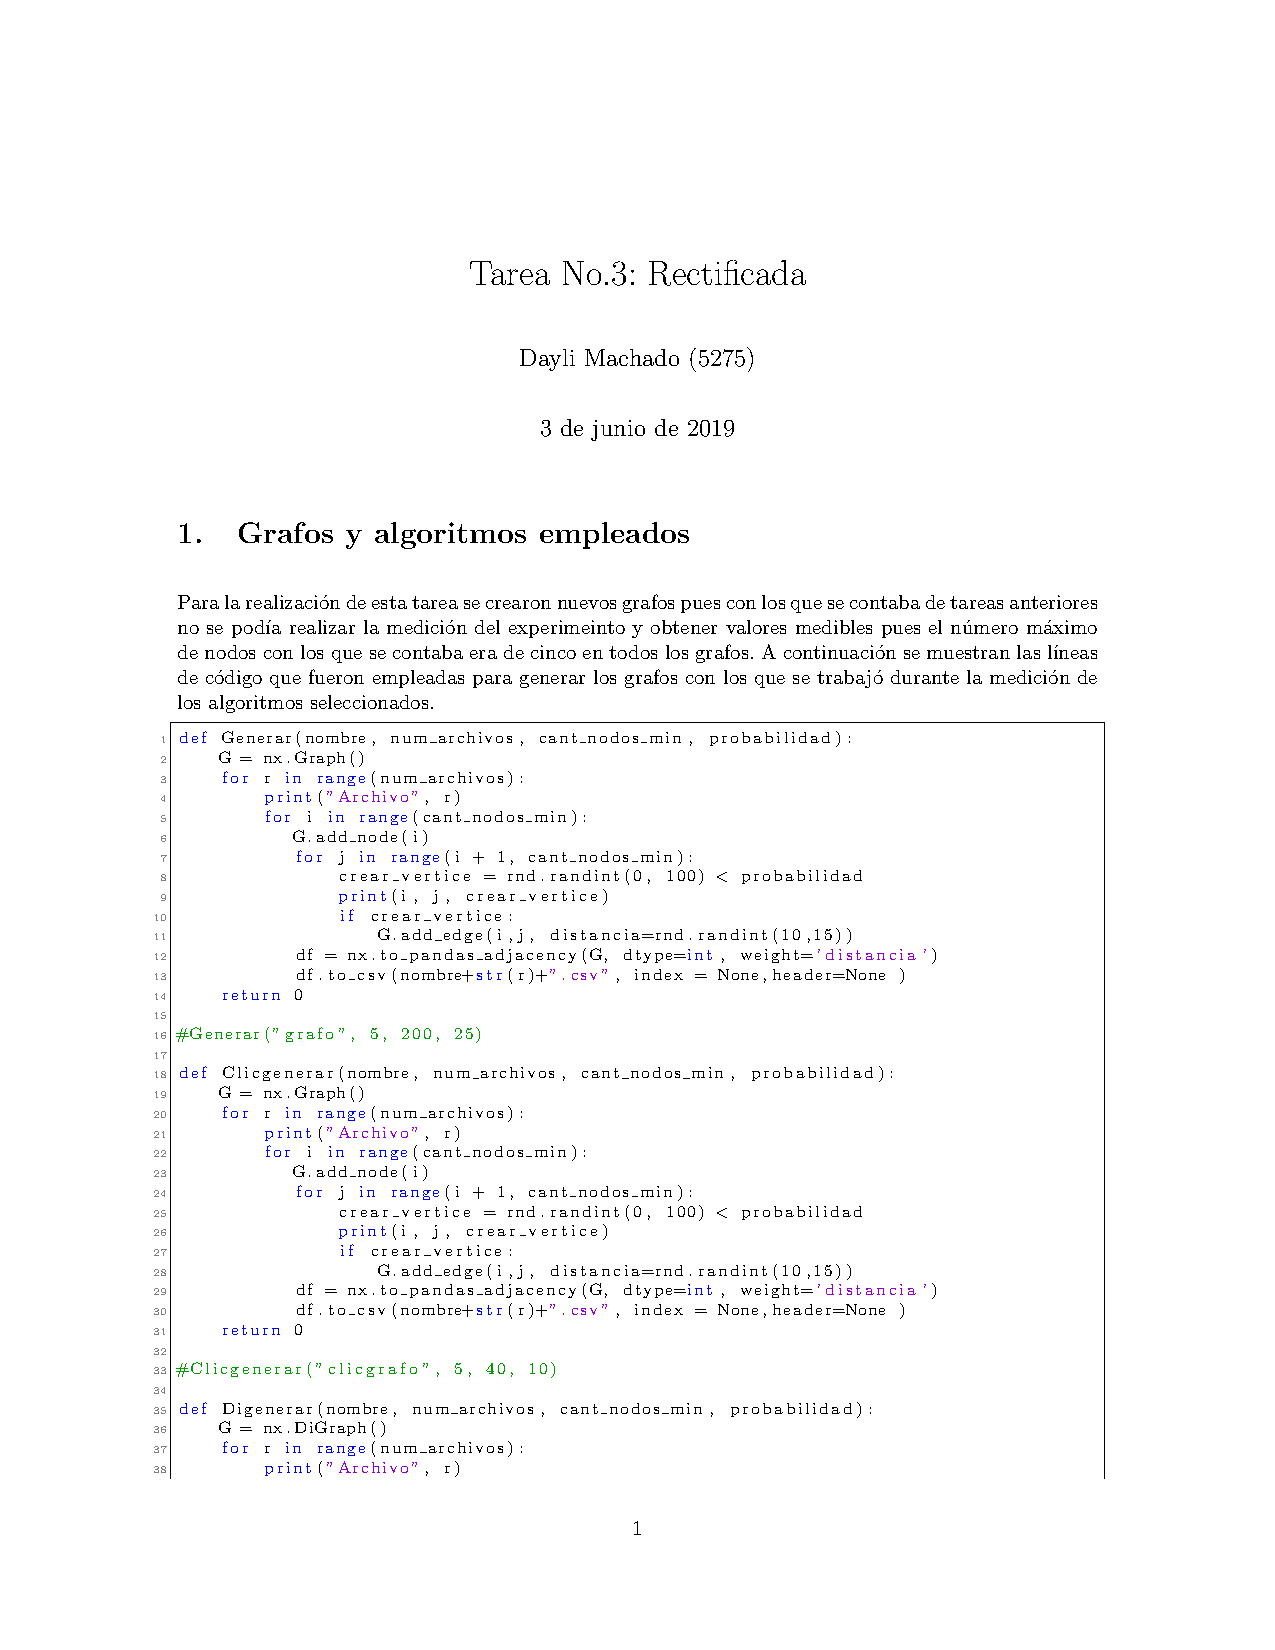
\includepdf[pages=1-13]{pdfrectificados/Tarea3_Rectificada.pdf}

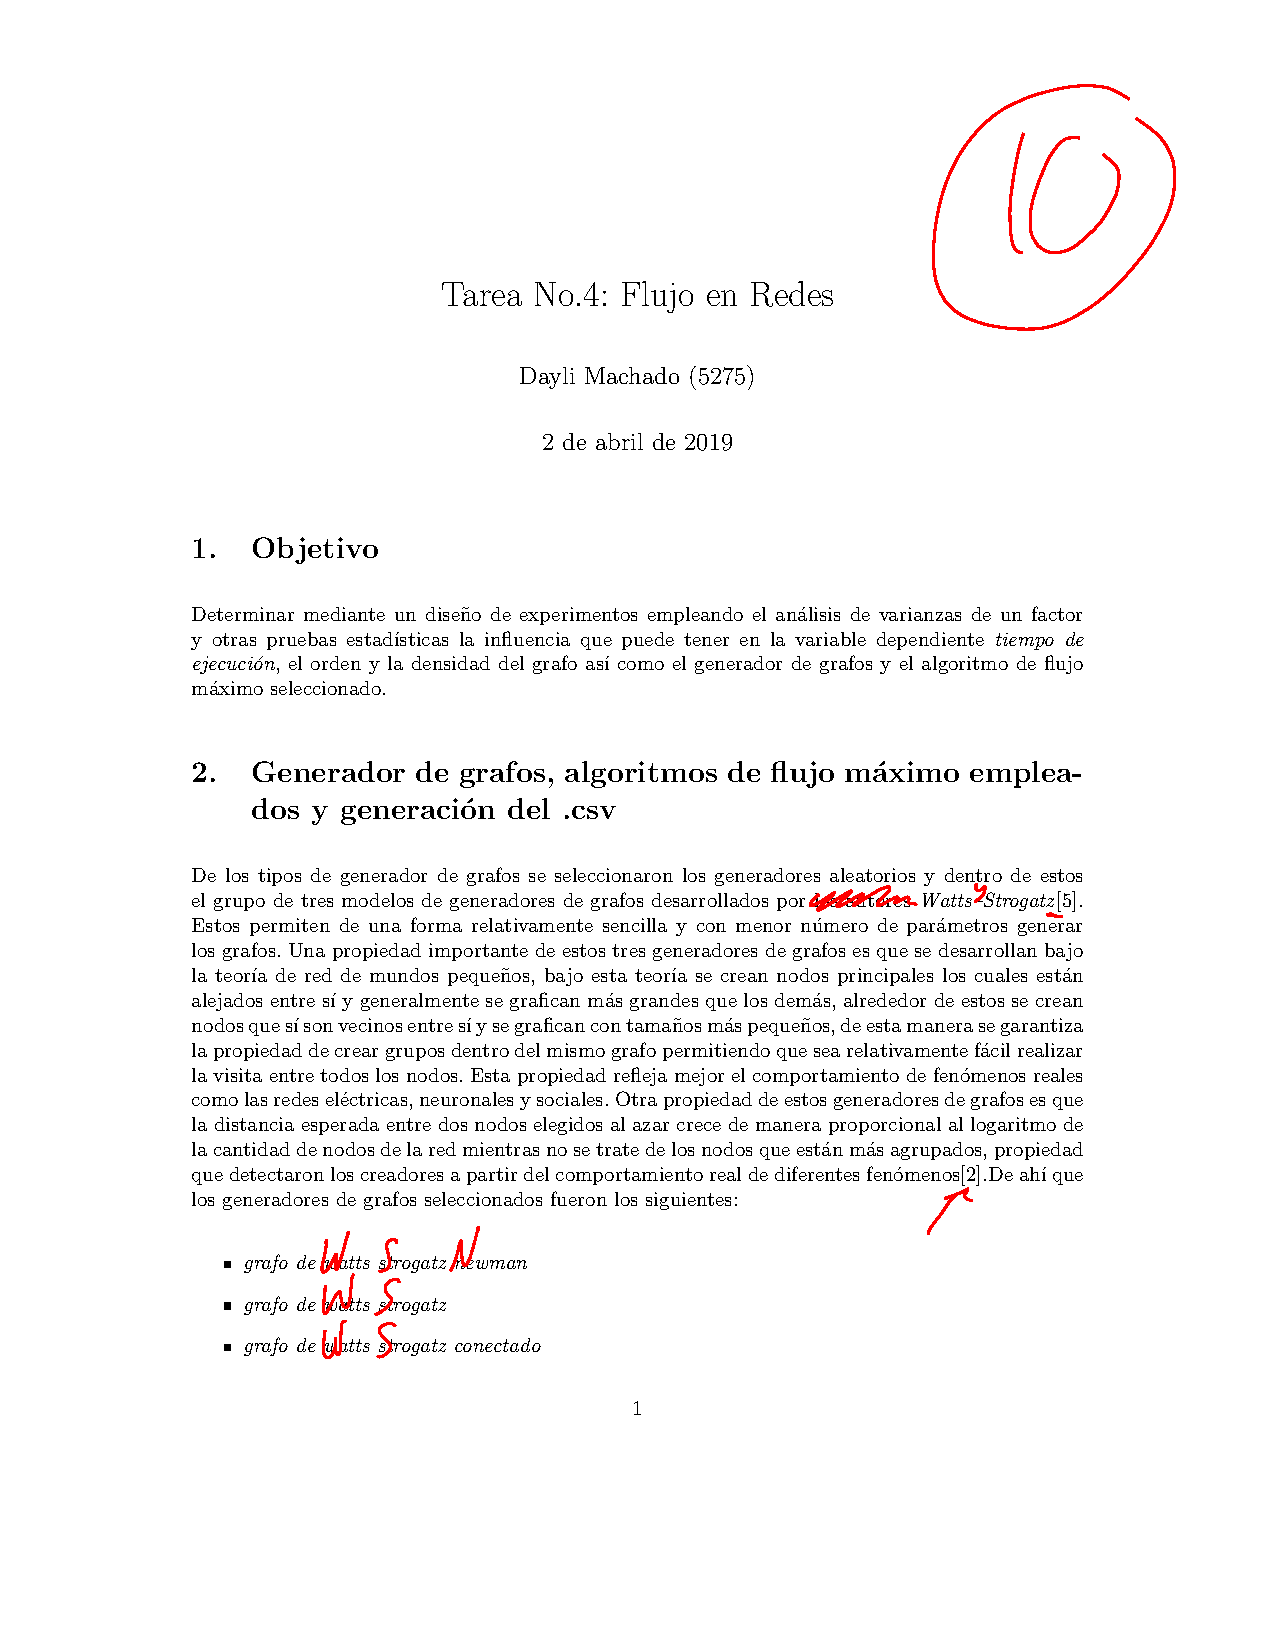
\includepdf[pages=1-13]{pdfrevisados/5275-4.pdf}
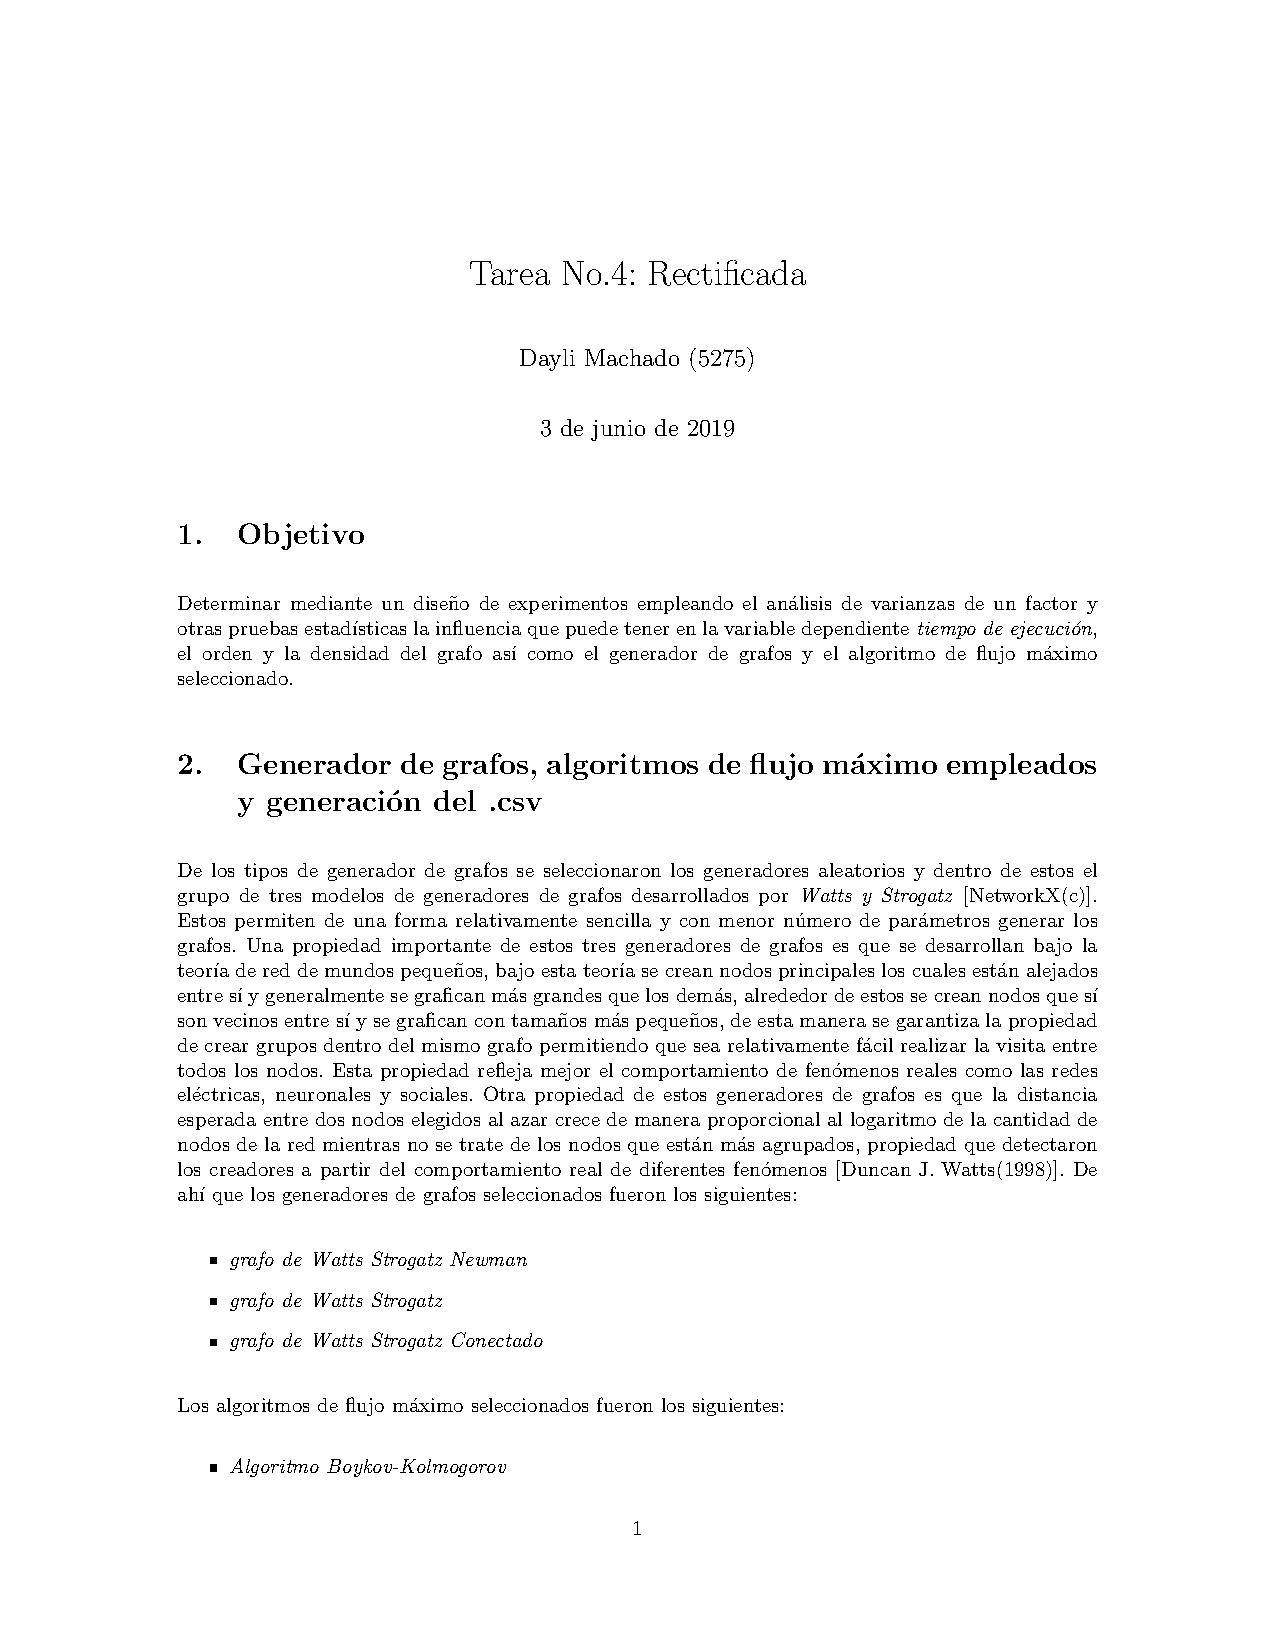
\includepdf[pages=1-11]{pdfrectificados/Tarea4_Rectificada.pdf}

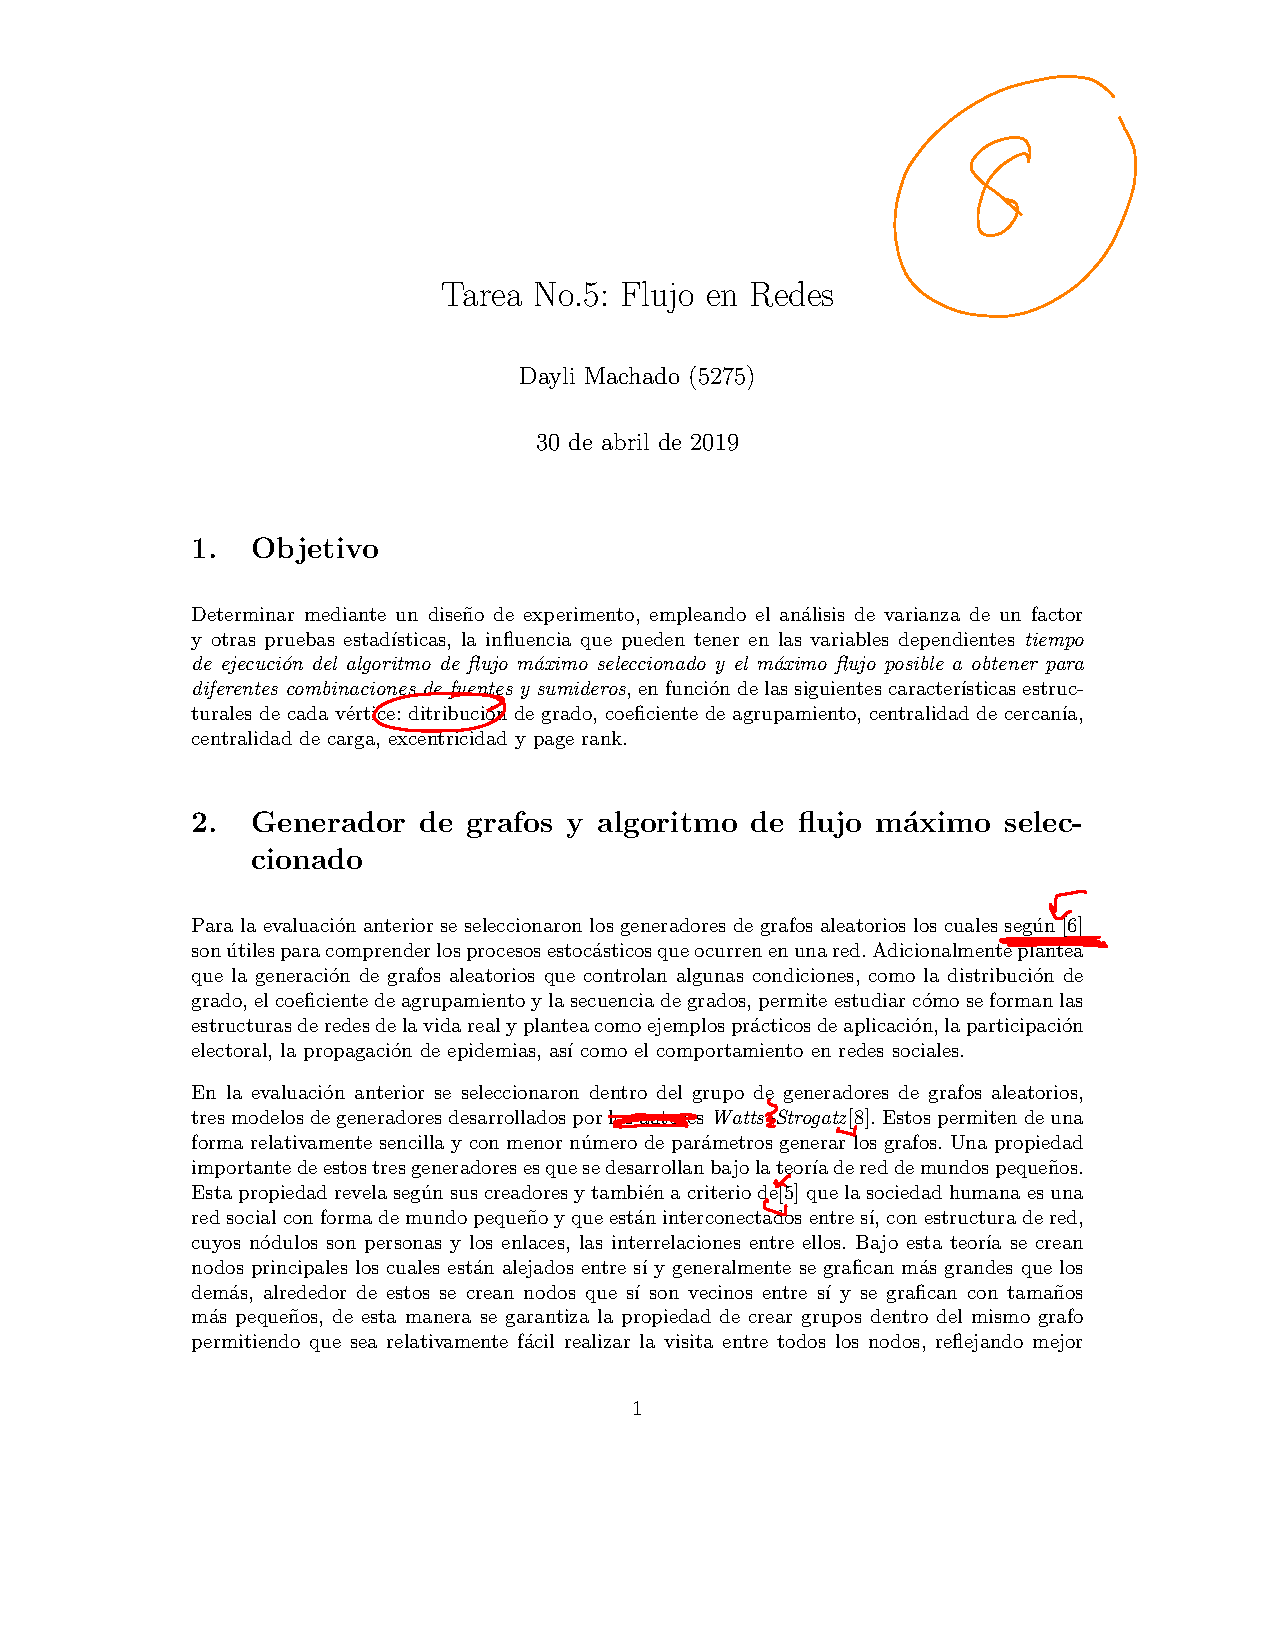
\includepdf[pages=1-29]{pdfrevisados/5275-5.pdf}
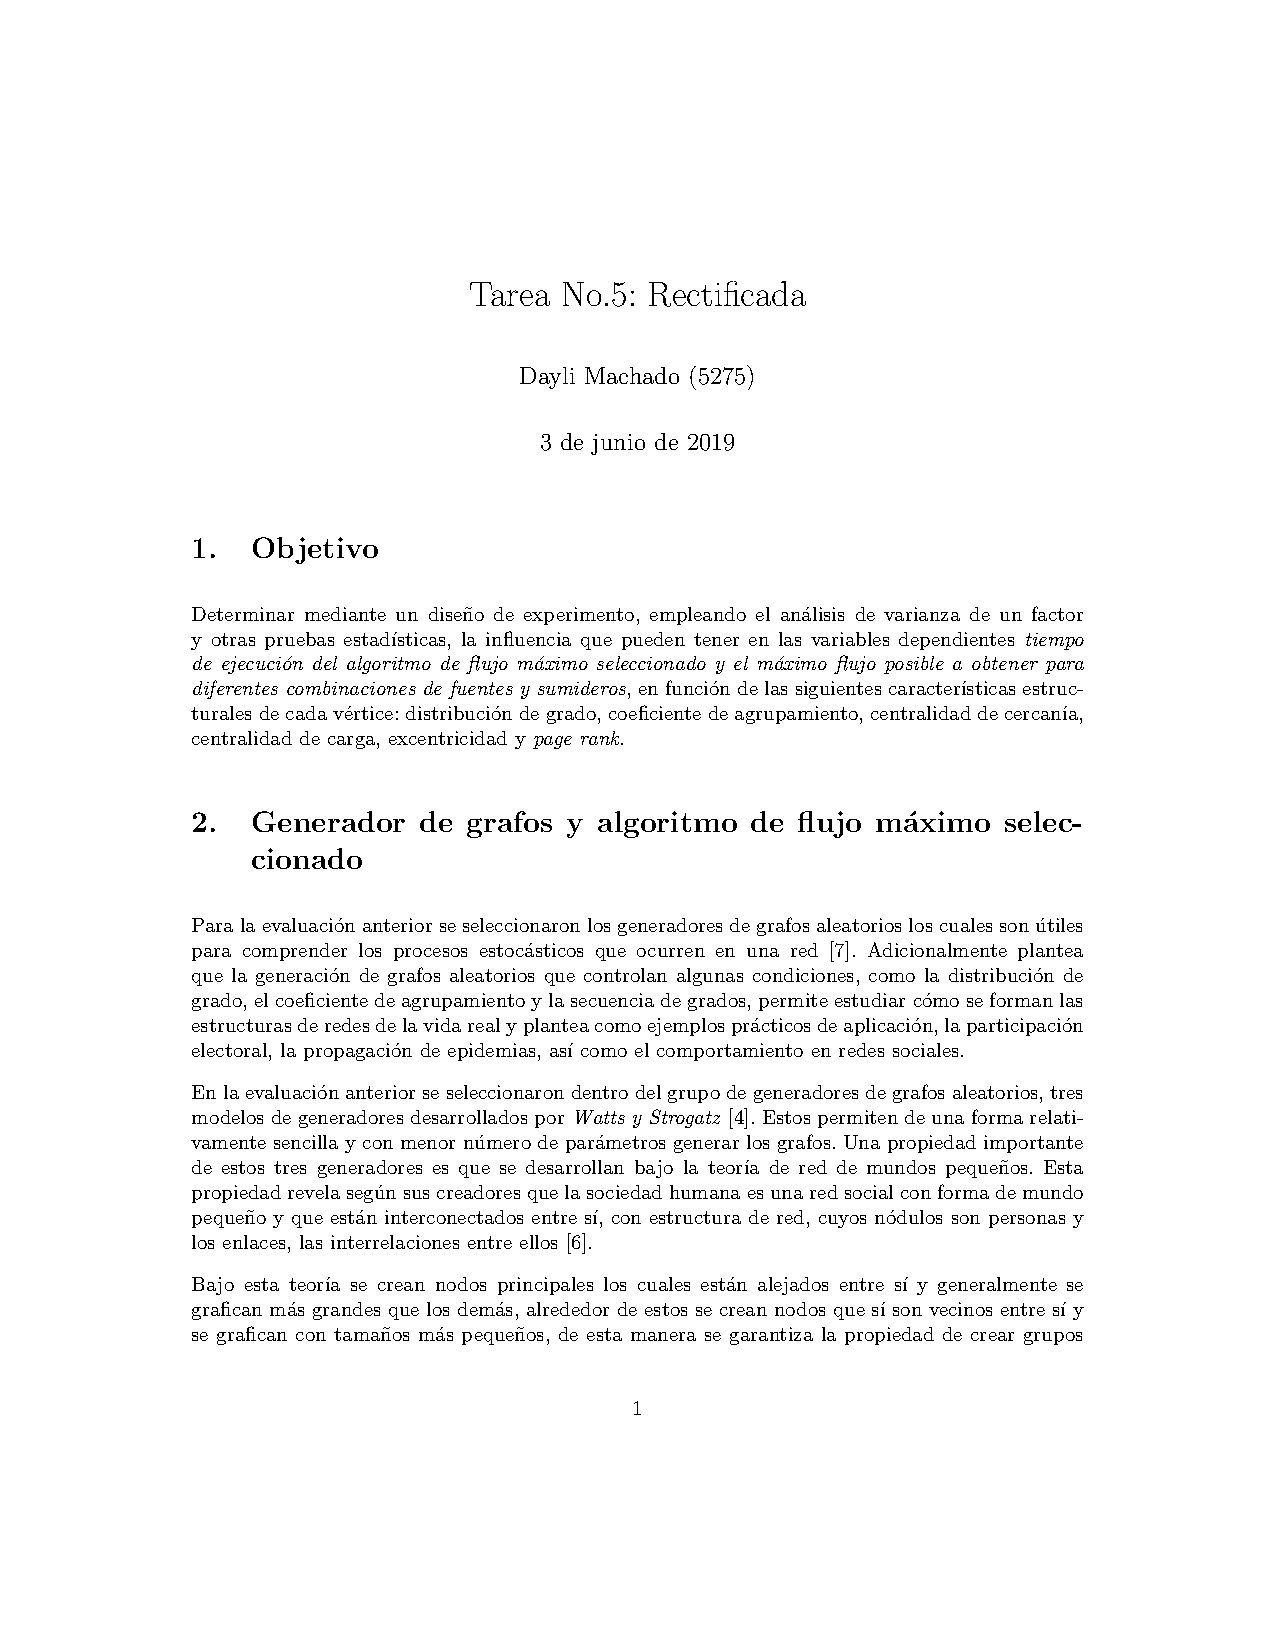
\includepdf[pages=1-30]{pdfrectificados/Tarea5_Rectificada.pdf}
\end{document}